% =====================================================================
%  Chapter 15 — The Target and the Forward Return
% =====================================================================

\chapter{The Target and the Forward Return}
\label{ch:target}

Everything in Part IV is an attempt to estimate one number per fund per
month: the expected forward return. This chapter defines the number,
states the convention that makes the forward return honest, and shows how
the horizon enters every other quantity in the book.

\section{The definition}

At formation date \(t\), the target for fund \(i\) is the total return
realised between \(t\) and \(t+h\):

\[
y_{i,t}^{(h)} = \prod_{k=1}^{h}\left(1 + r_{i,t+k}\right) - 1.
\]

It is a compounded forward return, not a sum, because the thing being
predicted is what an investor would have earned.

The monthly panel makes this a rolling product shifted backwards by the
horizon, so that row \(t\) holds the return realised between \(t\) and
\(t+h\):

\begin{equation}
\text{forward}_{t}^{(h)} = \left[\prod_{k=0}^{h-1}(1+r_{t+k})\right] - 1,
\qquad
\text{target}_t^{(h)} = \text{forward}_{t+h}^{(h)} .
\end{equation}

The shift is the whole mechanism of the look-ahead defence, and it is
worth being explicit about why. The rolling product as first written is
\emph{not} the forward return: it is the trailing return, because the
product runs forwards in the index but the data at row \(t\) only knows
about \(t\) and earlier. Shifting it back by \(h\) places, at row \(t\), the
return that will be realised between \(t\) and \(t+h\). A model trained on
the unshifted series would be predicting the past.

\begin{figure}[!htbp]
\centering
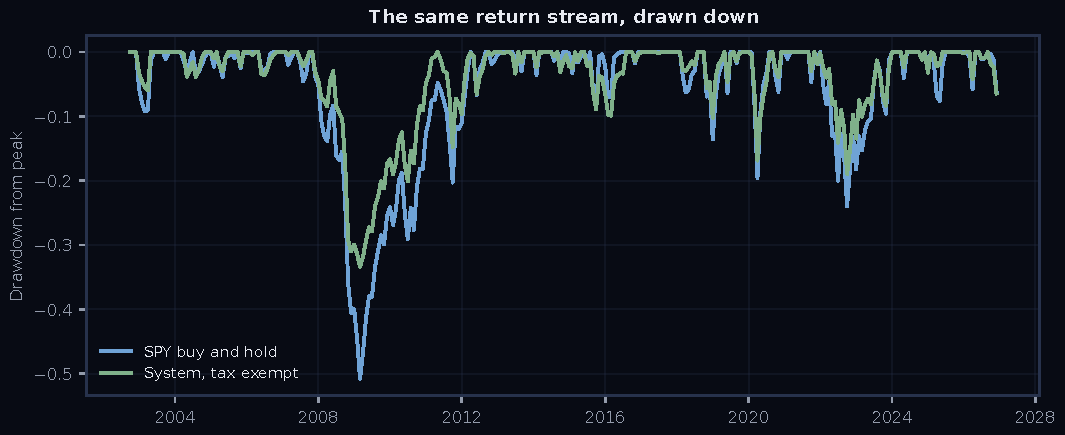
\includegraphics[width=\textwidth]{../figures/fig_drawdown.pdf}
\caption{The two accounts --- taxable and tax-exempt --- and the
benchmark, with the drawdown beneath. The gap between the two accounts is
the tax; the gap between the system and the benchmark is the subject of
Part VI.}
\label{fig:drawdown}
\end{figure}

\section{Two horizons, and why the book uses both}

The book's model set uses two horizons: one month and three months.

The one-month horizon is the natural one for a monthly rebalancing system
and it matches the data's native frequency, which means the training set
loses only one month of information at each formation date.

The three-month horizon is included for a substantive reason. It is a
different bet. A one-month forecast is dominated by short-horizon
reversal and by microstructure; a three-month forecast is long enough for
momentum to dominate and short enough to be actionable in a monthly
rebalancing scheme. If the two horizons' forecasts agree, the signal is
more likely to be about the asset than about the horizon. If they
disagree, the ensemble has to decide.

Including two horizons doubles the trial count, and the trial count is
expensive: every additional configuration raises the bar that the best
configuration has to clear to be distinguishable from luck. The book
accepts that cost because the alternative --- a single horizon --- would
embed a bet about the most contested parameter in the entire subject
inside the design of the ensemble, where it could not be examined.

\section{The units problem, and its resolution}

There is a subtlety that will destroy the estimates if it is ignored, and
it is the kind of thing that separates a careful implementation from a
plausible one.

A member with horizon \(h\) forecasts an \(h\)-month return. Its posterior
mean is therefore in \(h\)-month units and its posterior variance is in
\(h\)-month squared units. But the portfolio problem that the forecast
feeds into is a \emph{monthly} one: the covariance is estimated from
monthly returns, and the book rebalances monthly. Adding a three-month
variance to a monthly covariance, or comparing a three-month mean against
a monthly covariance, is dimensionally wrong, and it is wrong in a way that
is systematically harmful: it understates the three-month members' edge
by a factor of three and makes the two horizons incomparable, so the
ensemble is averaging quantities that are not the same quantity.

The book's resolution is to convert every member's forecast to a monthly
rate before it is combined:

\[
\mu^{(1)} = \left(1+\mu^{(h)}\right)^{1/h} - 1,
\qquad
v^{(1)} = \frac{v^{(h)}}{h^{2}}.
\]

The first is exact; the second is the first-order scaling of a variance
under a time change, and it is accurate to the order that matters for the
decision being made. The conversion happens \emph{before} the model-spread
term of Chapter 19 is added, so the spread between members is also
measured in monthly units and is comparable across horizons.

This is worth flagging as a general point, because the bug is a common
one and it is silent. Nothing in the output looks wrong. The system runs.
The equity curve looks reasonable. The problem is that the three-month
members are quietly doing less work than they should.

\section{What the target does not include}

Two omissions, both deliberate.

The target is a \emph{raw} forward return. It is not risk-adjusted, not
diversified, and not net of the cost of trading it. This is the correct
target for a model whose output is a per-asset expected return, because
the portfolio layer is where the risk adjustment happens: the Kelly solve
in Chapter 26 divides the expected excess return by the covariance and
subtracts the uncertainty of the estimate, which is precisely the
correction that would otherwise be missing.

The target is also not the return of the \emph{whole portfolio}. This is
the deepest limitation of the design and it deserves to be stated plainly.
A one-asset-at-a-time regression can express a view about a fund relative
to the other funds that exist alongside it; it cannot express a view about
the portfolio as a whole, because it does not model the portfolio.

The defence is that the model is never allowed to set the portfolio. It
sets a bounded tilt inside a sleeve whose total weight is fixed by
policy. The portfolio-level decisions --- how much risk, in which sleeve,
with what drawdown tolerance --- are made by the stated policy and by the
governor, and the model's influence on them is bounded by construction.

\begin{takeaway}[The target]
The target is the compounded \(h\)-month forward total return, formed by
shifting a rolling product backwards by \(h\), with \(h\) equal to one or
three months, converted to a monthly rate before the ensemble combines it.
It is a raw return: the risk adjustment and the trading cost are the
portfolio layer's business.
\end{takeaway}

\begin{keytakeaways}
\item The target is the compounded forward return realised between the
formation date and the formation date plus the horizon, obtained by
shifting a rolling product backwards by the horizon.
\item Two horizons are used, one month and three months, so that the
ensemble must reconcile a short-horizon and a medium-horizon bet, and the
cost of that choice is paid honestly in the trial count.
\item Every member's forecast is converted to a monthly rate before the
ensemble combines it, because the covariance is monthly; failing to do
this silently understates the three-month members by a factor of three.
\item The target is raw and per-asset, and the model is never permitted to
set the portfolio, which is what makes a per-asset regression an
acceptable design.
\end{keytakeaways}
